\subsection{Network, UI and Checkpoint Interface}
The Agent module is the heart of the the whole logic and data structure. It brings all gearwheels together and therefore, needs a special architecture as depicted in Figure~\hyperref[interface_overview]{3.4}.
For a more detailed overview over the dependencies of the abccore module see Figure~\hyperref[agent_dependencies]{3.5}
The Agent extends the class AgentMessageHandler which is responsible for handling messages from the Network.
This inheritance allows the Agent itself to actually handle messages from the network.
Sending own messages back to the network can be done over a special ChannelService which is given within the constructor of the AgentMessageHandler.

For the UI establishing the Agent also extends the LocalMessageHandler class. This class offers the UI multiple predefined method calls such as \texttt{send\_money} and the direct access to the Agent memory.
Updates can only be initialized on the UI side, the Agent itself has no opportunity to initialize a communication to the UI.

For the injection of new computed checkpoints the checkpoint service can call the method \texttt{inject\_checkpoint(ckpt)} which will overwrite the current state of the DAG.
Besides this the checkpoint service also has access to the Agents memory to be able to negotiate new checkpoints. 

\begin{figure}[h]
	\centering
	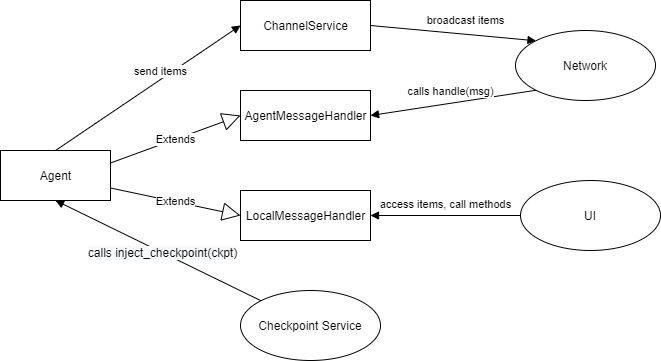
\includegraphics[scale=0.7,trim={1cm 18.5cm 0cm 0cm}, origin=c, clip ]{figures/drawio/class_diagram_overview.pdf}
    \footnotesize{Figure~\hyperref[interface_overview]{3.4}:~Interface~Overview~from~an~Agents~Side}
    \label{interface_overview}
\end{figure}

\begin{figure}[h]
	\centering
	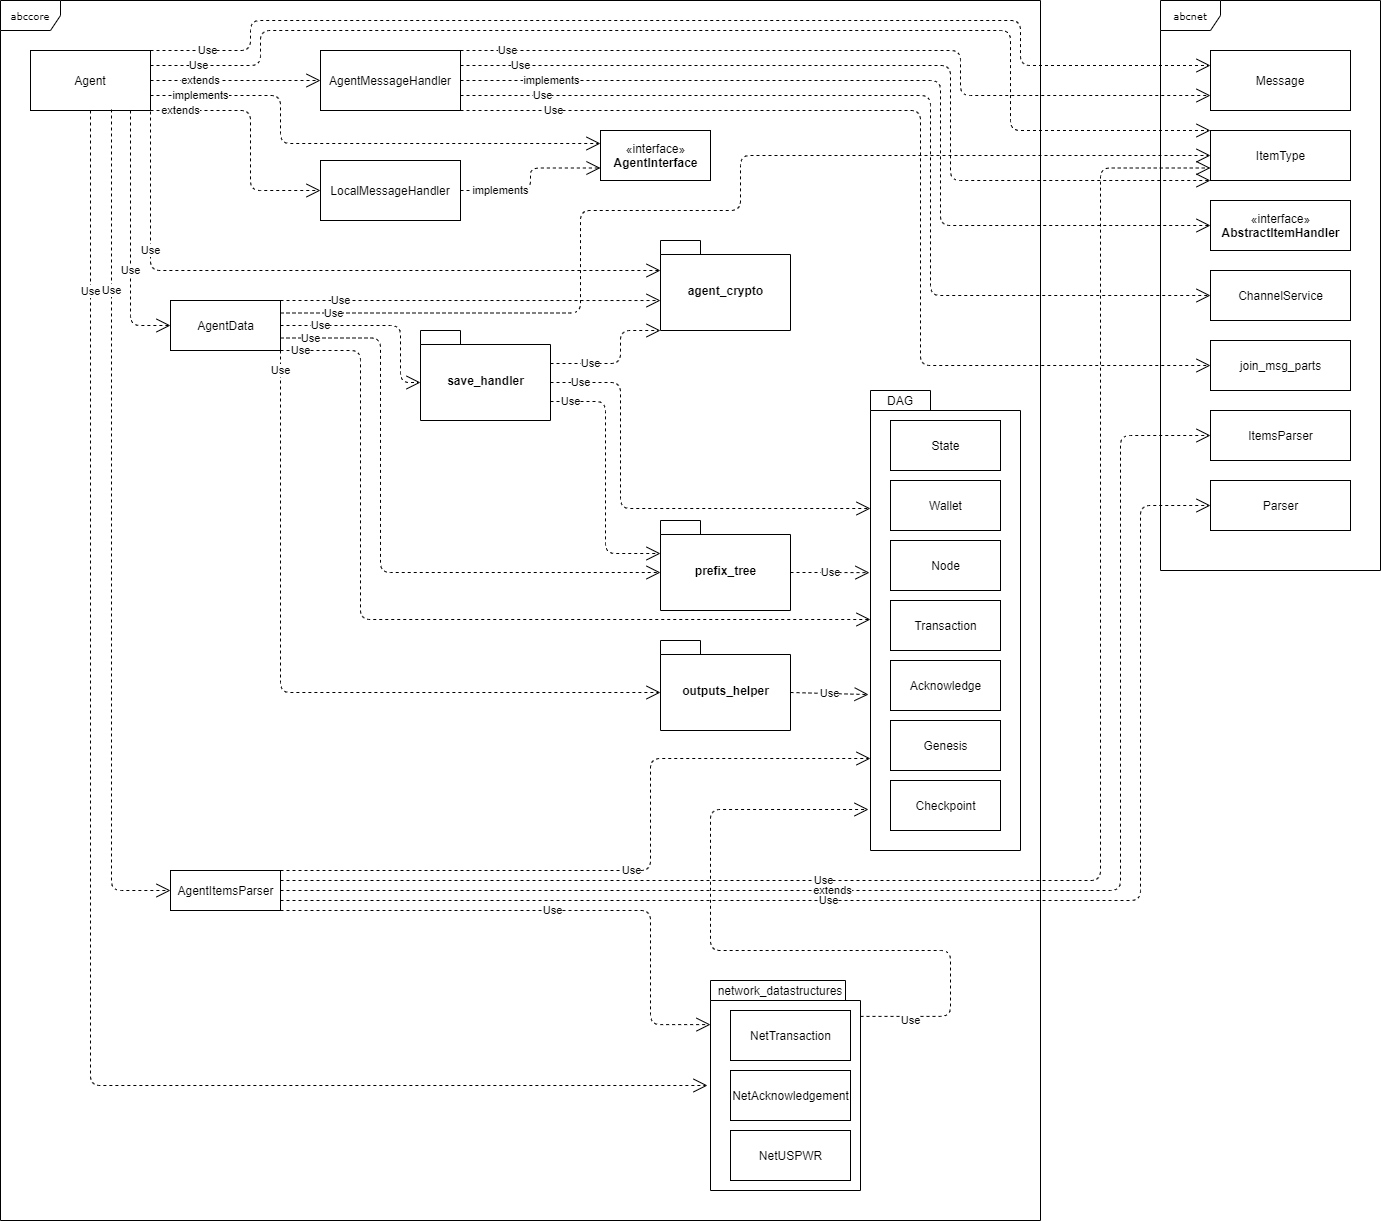
\includegraphics[scale=0.45, trim={0cm 0cm 0cm 0cm},clip]{figures/drawio/agent_dependencies.pdf}
	\footnotesize{Figure~\hyperref[interface_overview]{3.5}:~Agent~Dependency~Diagram}
	\label{agent_dependencies}
\end{figure}


\subsection{Data Preparation for the Network-Agent Interface}
\label{data_prep}
Our implementation of the ABC-protocol is build for a distributed environment. Since all communication and messages are generally broadcasted to the whole network sending each new acknowledgement, transaction or unspent-wallet-request message one by one can harm the throughput of the whole network.
Further, directly reacting to new messages from the network can lead to much more traffic. The Push-and-Pull protocol we are using for the network first provides checklists of IDs for the network so remote agents can request these new items on demand.
If an agent receives a new checklist of new item-IDs it might request the network for the actual content by sending a fetch-item list which includes the IDs of the requested items as well.
Eventually, if an remote agent has the underlying content to the corresponding ID this remote agent will send the content within a item list.
If we now imagine a system where each remote agent directly reacts to new messages the whole network would be overflowed with checklists, fetch-item lists and item-lists each consisting of single elements. Additionally, messages can be received in a different order they were send due to possible delays on the network layer, so further additional requests for items which are already sent to the network are created.

\begin{figure}[h]
	\centering
	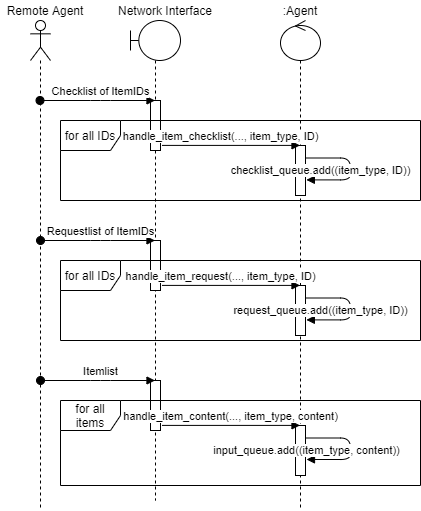
\includegraphics[scale=0.8,trim={0cm 15cm 10cm 0cm}, origin=c, clip ]{figures/drawio/sequence3.pdf}
    \footnotesize{Figure~\hyperref[input_queues]{3.6}:~Checklist,~Requestlist~and~Itemlist~Handling}
    \label{input_queues}
\end{figure}

To prevent this overflowing with messages the Agent class first collects all incoming messages in the \texttt{input\_queue} for all items of received item lists, in the \texttt{request\_queue} for all item IDs of received fetch-item lists and in the \texttt{checklist\_queue} for all item IDs of received checklists as pictured in Figure~\hyperref[input_queues]{3.6}.


For the \texttt{checklist\_queue} and the \texttt{request\_queue} we use \texttt{set()} as datatype, so duplicates e.g. received due to different checklists of different agents are directly eliminated.
Since we also want to prevent spamming attacks by the agent itself created by fast item-generation like transactions we use this system not only for incoming items but for outgoing items as well.
The Agent first collects all created items like transactions or acknowledgements and prepares the outgoing checklist, fetch-item list and item-list.
After a certain amount of time the BaseApp will call the method \texttt{perform\_maintenance()} of the Agent which basically works through all the incoming items to make method calls for further proceeding and all the outgoing lists to propose new items and item requests to the network.



To actually  send items to the network as already mentioned in Section~\ref{local_data_handling}  the Agent first has to prepare and transform them.
For this purpose the Agent makes use of the datatypes NetTransaction, NetAcknowledgement and NetUSPWR (= Net-Unspent-Wallet-Request).
These are necessary because the for the internal data structure used objects do not include necessary properties to be encodeable and decodeable for the network purpose in a useful manner.
Only these three "Net"-item types can be send from an Agent instance.


\subsection{Replay Function}
During the runtime of our distributed system new agents may join or will go offline to join again to a later point in time.
Since new agents only know the genesis and previously offline agents only know the latest status before they turned offline we had to implement a replay functionality to our system.
First, after start-up the checkpoint service will get the latest checkpoint from the network and inject it into our Agent instance.
Now the Agent instance has to replay all transactions since this checkpoint or, if this state is actually newer, from his last state on.
To do so the Agent instance collects all unspent wallets and sends them to the network with help of the specific NetUSPWR datatype as described in Section~\ref{data_prep}.
If a remote Agent instance will receive such a request it will resend all transactions and acknowledgements which have been sent after the by the NetUSPWR specified unspent-wallets.
The previously offline Agent can now just add all objects he does not know to his local AgentData structure.


\subsection{Example Run Throughs}

\subsubsection{Example: Sending Money}
In the following we will show an example run through of the \\
\texttt{send\_money(value,recipient,validator)} method which is also shown in \\Figure~\hyperref[send_money]{3.7}.
This method is called if a new transaction is initialized within the UI.
The call will then be forwarded to the AgentData class.
Since wallets are handled like piggy banks and can only be used as whole we can not just take the needed money of one wallet.
Instead, we are processing our owned wallets and set up a wallet set which is able to pay the needed value and the additional fee which will be needed for submitting the transaction.
This is done by the method \texttt{get\_transaction\_set(value)}.
Further, the resulting wallets will most probably not match the exact value we need for the transaction and the additional fee.
Therefore, we use the method \texttt{outputs\_helper} to actually compute the wallets we want to spend to the transaction's recipient and one wallet which will set up a new wallet for the Agent itself to store the rest of the input wallets money which has not been used.
After the input and output wallets have been successfully computed the Agent can now setup the transaction itself.
To proof the ownership of the input wallets the Agent now signs the transaction with all secret keys which belong to the owner public keys of the input wallets.
The transaction can only be validated successfully later if the transaction is signed by each owner key of these input wallets.
After the transaction is initialized the Agent itself will create a NetTransaction object to propose the new transaction to the network.
This new NetTransaction item is now added to the outgoing checklist queue as described in Section~\ref{data_prep}.
Now, the Agent will acknowledge the transaction with all of his keypairs and therefore, its whole amount of stake.
Since transactions are only confirmed if at least $\frac{2}{3}$ of the stake in the whole network acknowledged it, it is important to actually acknowledge this new transaction with as much own stake as possible.
Each created Acknowledge object will have exactly one signature, namely the signature of the keypair this acknowledgements public key hints to.
After the AgentData class has acknowledged the new transaction with all of its keys it will return a list of the newly created acknowledgements to the Agent instance.
The process of acknowledging new transactions we just ran through even is the same for new transactions received by the network. Of course validation is a very important part here as well (even if the transaction is created by ourself) but this would go too much into deep.
Now, similar as for the transaction object, the Agent will create several NetAcknowledgement objects to prepare the Acknowledge objects for sending over the network.
Again, the newly created NetAcknowledgement objects are added to our outgoing checklist so they can be actually send within the next \texttt{perform\_maintenance()} call.
Since transaction creation, validation and acknowledgement creation is now complete the \texttt{send\_money(...)} call is finished.
By sending the transaction and the own acknowledgements within the same checklist in the \textbf{next} \texttt{perform\_maintenance()} call we can again reduce the number of single messages in the network.


\begin{figure}[h]
	\centering
	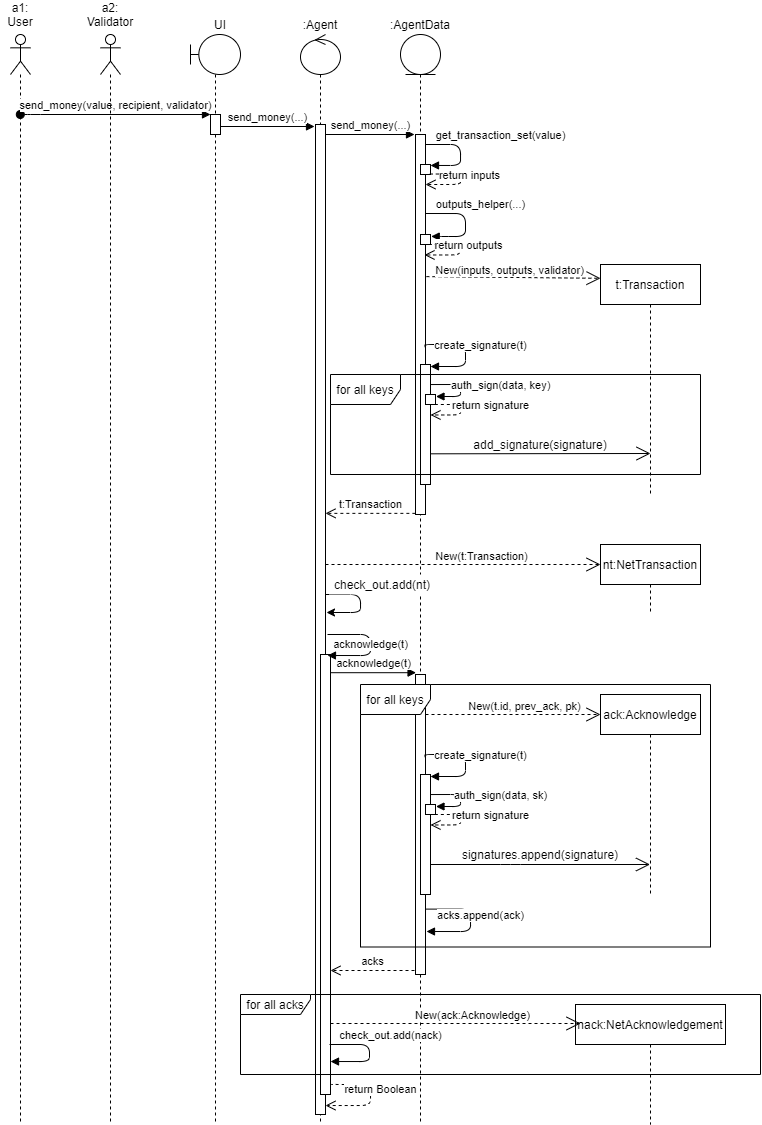
\includegraphics[width=0.8\textwidth, trim={0cm 0cm 0cm 0cm},clip]{figures/drawio/sequence1.pdf}
	\footnotesize{Figure~\hyperref[send_money]{3.7}:~"Send~Money"~Run~Through}
    \label{send_money}
\end{figure}

\subsubsection{Example: Generating/Adding new Keypairs}
The following run through is shown in Figure~\hyperref[sequence2]{3.8}.
If the user wants to generate a new keypair he can click the button "Generate Keys" in the UI.
The UI will forward the call to the corresponding Agent instance which further forwards it to AgentData and the "cryptography" module \cite{pypi_crypt} related methods in the "agent\_crypto.py".
After generation the key will be added to the keyset by the AgentData instance of the Agent.
After the key has been added the UI will call an update from the Agent to actually show the newly created keypair in the UI.

If the user wants to add a new keypair manually, e.g. because he wants to synchronize his wallets over multiple devices, he can just press the "+" button in the UI and enter the secret key he wants to add in hexadecimal representation.
The UI will forward the call to agent, which will further forward it to the AgentData instance to actually add the newly created secret key to the database.
For the keygeneration and signatures we use elliptic curve Diffie-Hellmann Ed25519 of the open source "cryptography" library \cite{pypi_crypt}.
Since this public key encryption scheme allows to compute the public keys out of the private key submitting only the private key is sufficient to add the whole keypair to the keyset of AgentData.


\begin{figure}[h]
	\centering
	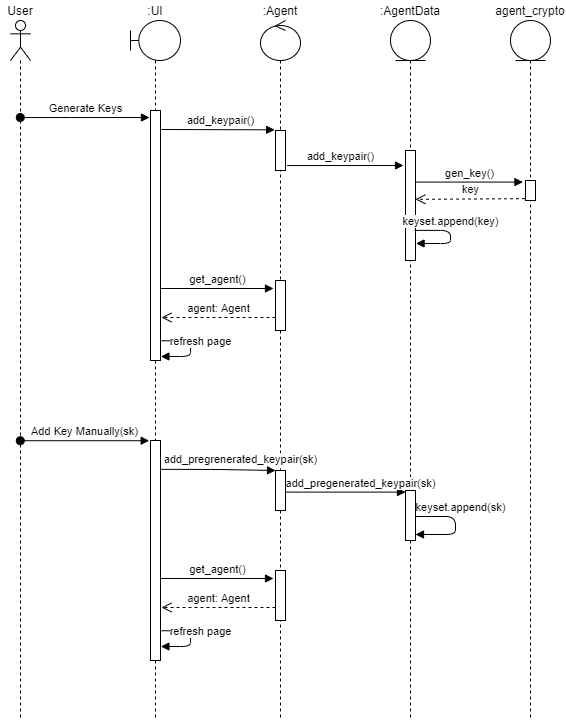
\includegraphics[width=0.8\textwidth, trim={0cm 0cm 0cm 0cm},clip]{figures/drawio/sequence2.pdf}
	\footnotesize{Figure~\hyperref[sequence2]{3.8}:~"New~Keypair"~Run~Through}
	\label{sequence2}
\end{figure}